\documentclass[10pt]{article}
\usepackage{icmlko}

\icmlmeta{IP 파운데이션 월드모델}{324}{마흔셋에서 열을 골랐더니 하나가 벌었다}{선별기를 원천 레코드로 넓혔다 --- 출처가 74\%를 막고, 남은 열이 검사를 다 통과하고, 그중 하나만 번다}

\begin{document}

\twocolumn[
\icmlheader

\begin{abstract}
노트 323이 ``넷째 축을 지어 검사가 또 갈리나 보라''를 남겼다. 노트 321의
선별기는 축 파일만 훑었으니 \textbf{원천 레코드}(\texttt{*\_records.json})로
넓혔다. 검사 ①③④ 를 통과하는 후보가 \textbf{마흔셋} 나왔다 --- 그리고
\textbf{출처가 서른둘(74\%)을 막는다}: 라벨 자체(\texttt{y\_positive} ·
\texttt{y\_backers} $\ldots$) · 지금 긁은 스냅샷(\texttt{favourites} ·
\texttt{mean\_score} · \texttt{sales\_point}, 노트 224) · 식별자
(\texttt{title\_id} $\ldots$ 시간과 붙는다) · \texttt{finished}(노트 255) ·
쌓이는 것(\texttt{n\_episode} · \texttt{n\_tag}). \textbf{통계만으로는 못
고른다.} 남은 열하나 중 검사 ② 를 돌릴 수 있는 \textbf{열이 전부 5/5} 이고
전부 사전이다. \textbf{열을 다 지어 쟀다.} 결과 --- \textbf{축을 받은 다섯
도메인 중 하나만 번다}: 펀딩 $+$0.1320($t{=}2.05$) · 모바일 $+$0.0086 ·
세계애니 $+$0.0058 · 웹툰 $-$0.0061 · \textbf{애니 $-$0.0329}($t{=}{-}2.16$,
두 실행 다). 판은 $-$0.0096 / $-$0.0027 이고 \textbf{어느 도메인도 문턱
($|t|{>}2.81$)을 안 넘는다.} \textbf{그래서 노트 323의 ``검사 넷이 정확히
갈랐다''는 $n{=}3$ 의 요행이었고 노트 322의 표제가 $n{=}10$ 에서 선다} ---
\textbf{검사는 거르지 줄 세우지 못한다.} 덤으로 시장팝업이 한 실행에서
$-$0.1231 이었다가 다른 실행에서 $-$0.0014 다 --- \textbf{축을 하나도 안
받은 도메인의 큰 수는 잡음이다}(노트 316).
\end{abstract}
]

\section{원천으로 넓혔다}

노트 321의 선별기가 축 파일에서 후보 셋을 찾았고 그중 하나를 지었다.
\textbf{원천 레코드}는 훨씬 넓다 --- 축 파일은 그것에서 뽑은 것이다.

\begin{center}\footnotesize
\begin{tabular}{lr}
\hline
검사 ①③④ 통과 후보 & \textbf{43} \\
\hline
출처가 막음 & \textbf{32 (74\%)} \\
\quad 라벨 자체 & 7 \\
\quad 지금 긁은 스냅샷(노트 224) & 7 \\
\quad 식별자(시간과 붙는다) & 5 \\
\quad \texttt{finished}(노트 255) & 1 \\
\quad 쌓이는 것 · 기타 & 12 \\
\hline
남은 사전 후보 & 11 \\
검사 ② 를 돌릴 수 있고 5/5 & \textbf{10} \\
\hline
\end{tabular}
\end{center}

\textbf{선별기가 마흔셋을 주고 사람이 열하나로 줄인다.} 노트 323의 규약
(``도구를 만들었으면 부르라'')의 짝이다 --- \textbf{도구는 통계를 보고
시점은 사람이 안다.}

\paragraph{지은 열} \texttt{mob\_advisory} · \texttt{mob\_ngenre} ·
\texttt{mob\_nlang}(모바일) · \texttt{wt\_agetype}(웹툰) ·
\texttt{ani\_quarter} · \texttt{ani\_studio}(애니) · \texttt{wa\_ngenre} ·
\texttt{wa\_source} · \texttt{wa\_studio}(세계애니) ·
\texttt{fund\_maxprice}(펀딩). 눈금은 범주${=}$집단 크기 순 · 수치${=}
$\texttt{rankdata} 백분위(노트 292의 동률 단언 포함). \textbf{라벨을
안 본다.}

\section{하나만 번다}

\begin{figure*}[t]
\centering
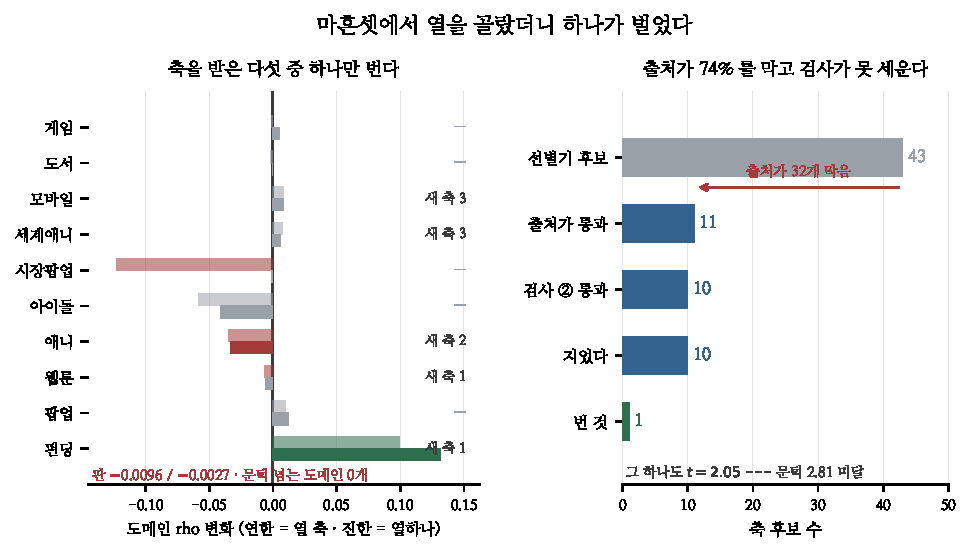
\includegraphics[width=\textwidth]{figs/ten.pdf}
\caption{왼쪽 --- 도메인별 변화(연한 막대 열 축 · 진한 막대 열하나).
오른쪽 --- 후보가 걸러지는 깔때기.}
\end{figure*}

\begin{center}\footnotesize
\begin{tabular}{lrrrrr}
\hline
도메인 & 새 축 & 열 축 & $t$ & 열하나 & $t$ \\
\hline
게임 & --- & $-$0.0010 & $-$0.10 & $+$0.0056 & $+$0.55 \\
도서 & --- & $-$0.0017 & $-$0.11 & $-$0.0005 & $-$0.03 \\
모바일 & 3 & $+$0.0087 & $+$0.46 & $+$0.0086 & $+$0.46 \\
세계애니 & 3 & $+$0.0075 & $+$0.63 & $+$0.0058 & $+$0.49 \\
시장팝업 & --- & $-$0.1231 & $-$1.79 & $-$0.0014 & $-$0.04 \\
아이돌 & --- & $-$0.0583 & $-$1.15 & $-$0.0408 & $-$0.71 \\
\textbf{애니} & 2 & \textbf{$-$0.0348} & \textbf{$-$2.18} & \textbf{$-$0.0329} & \textbf{$-$2.16} \\
웹툰 & 1 & $-$0.0069 & $-$1.76 & $-$0.0061 & $-$1.50 \\
팝업 & --- & $+$0.0102 & $+$0.50 & $+$0.0124 & $+$0.61 \\
\textbf{펀딩} & 1 & \textbf{$+$0.0998} & $+$1.67 & \textbf{$+$0.1320} & \textbf{$+$2.05} \\
\hline
\textbf{판} & 10 & \textbf{$-$0.0096} & & \textbf{$-$0.0027} & \\
\hline
\end{tabular}
\end{center}

\textbf{축을 받은 다섯 중 하나만 번다.} 그리고 \textbf{어느 도메인도 문턱
($|t|{>}2.81$)을 안 넘는다} --- 양쪽 다.

\paragraph{펀딩의 두 축이 겹친다} \texttt{fund\_cat} 혼자 $+$0.1173(노트 309) ·
\texttt{fund\_maxprice} 혼자 $+$0.0998 · 둘 다 $+$0.1320. \textbf{더해지지
않는다.} 펀딩에서 회수할 수 있는 것이 $\rho$ 0.13 쯤이고 두 축이 각자
그 대부분을 잡는다.

\paragraph{애니는 세 축이 다 해롭다} \texttt{anime\_medium}(노트 321)
$-$0.0091 · $+$\texttt{ani\_quarter} · \texttt{ani\_studio} 로
$-$0.0329($t{=}{-}2.16$). \textbf{두 실행에서 같다.} 애니는 이미 축이
스물셋인데 셋을 더해서 나빠졌다.

\section{그래서 노트 322가 옳았다}

\begin{center}\footnotesize
\begin{tabular}{lll}
\hline
노트 & 주장 & 지금 \\
\hline
322 & 검사는 줄 세우지 못한다 & \textbf{$n{=}10$ 에서 선다} \\
323 & 검사 넷이 셋을 갈랐다 & \textbf{$n{=}3$ 의 요행} \\
323 & \texttt{mkt\_cat} 은 ③ 탈락 & \textbf{그대로 옳다(사실 정정)} \\
\hline
\end{tabular}
\end{center}

노트 323이 노트 322의 \emph{전제}를 고친 것은 옳았다 --- \texttt{mkt\_cat} 은
정말 검사 ③ 에서 떨어진다. 그런데 거기서 \textbf{``검사 넷이 셋을 정확히
갈랐다''로 나아간 것이 성급했다.} 표본 셋으로 규칙을 세웠고, 열로 재니
안 선다.

\begin{center}\small
\textbf{검사는 아래를 자르고 위를 못 세운다}
\end{center}

출처는 74\%를 막았다 --- \textbf{거르기는 강력하다.} 그런데 남은 열이
전부 ①②③④ 를 통과하고도 아홉이 못 벌었다.

\section{덤 --- 축을 안 받은 도메인의 큰 수}

시장팝업이 한 실행에서 $-$0.1231($t{=}{-}1.79$)이고 다른 실행에서
$-$0.0014($t{=}{-}0.04$)다. \textbf{시장팝업은 새 축을 하나도 안 받았다.}
아이돌도 $-$0.0583 $\to$ $-$0.0408 로 흔들린다.

\textbf{노트 316이 말한 그대로다} --- 얇은 도메인의 큰 수는 읽으면 안 된다.
\textbf{한 실행만 봤으면 ``열 축이 시장팝업을 $-$0.12 죽인다''를 썼을
것이다.}

\paragraph{배포} 두 축 세트 다 규칙 ①②를 통과한다(판이 띠 안 · 나빠진
도메인이 문턱 안 넘음). \textbf{그런데 안 쓴다} --- 판이 $-$0.0096 이고
버는 것이 문턱 아래다. \texttt{fund\_maxprice} 를 \texttt{fund\_cat} 에
더하는 것도 $+$0.0147 로 펀딩 문턱(0.13)의 9분의 1이다.

\paragraph{남은 것}
\begin{center}\small
\begin{tabular}{ll}
\hline
갈래 & 왜 \\
\hline
애니는 왜 축을 싫어하나 & 셋 다 해롭다 \\
펀딩 0.13 의 천장 & 두 축이 같은 것을 잡는다 \\
검사 다섯째가 있나 & 넷으로는 못 세운다 \\
축 대신 행 & 오늘 축 열둘이 판을 못 올렸다 \\
\hline
\end{tabular}
\end{center}

\paragraph{규약} \textbf{규칙을 세우려면 표본을 세라.} 노트 323이 세 축으로
``검사 넷이 갈랐다''를 썼고 하루 만에 열로 무너졌다 --- 오늘 아침 노트 314가
\emph{같은 잘못}(못 가르는 값들의 순서)으로 노트를 물렀는데, 저녁에 표본 셋
짜리 규칙을 세웠다. \textbf{잣대를 만든 날에도 자기에게 안 댔다.}
그리고 \textbf{짓는 것은 재는 것보다 싸다} --- 열 축을 짓는 데 한 시간,
재는 데 십 분이었고, 그 십 분이 ``검사가 예측한다''를 무너뜨렸다.
\textbf{의심되면 지어서 재라.}

\end{document}
